\chapter{Приложения моделей близости ключевых слов} \label{chapt1}
В настоящем разделе рассматриваются реальные задачи и системы, в которых применяются программные реализации алгоритмов. 
Рассматривается задача поиска эксперта в области, определяемой заданным запросом из ключевых слов.
Также описывается использование тезауруса ключевых слов для задачи улучшения ранжирования в поисковой составляющей интеллектуальной системы <<ИСТИНА>>.
В конце раздела представлены выводы, а также дальнейшее направление в применении разработанных программных комплексов в реальных приложениях.

\section{Решение задачи поиска экспертов} \label{expert_search}
\subsection{Постановка задачи}
Дано множество наборов ключевых слов $W_X$ и объектов информационной системы $X$, а также множество $Q$ запросов к системе. Обозначим за $W$ множество всех уникальных ключевых слов из всех наборов $W_X$. Каждый элемент $x_i \in X$ множества объектов ассоциирован с набором ключевых слов $W_i = \{w_{i_0}, w_{i_1}, ..., w_{i_{n_i}} \} \in W_X \in 2^W$. Точно также каждый запрос $q_j \in Q$ связан с некоторым набором ключевых слов $W_j = \{w_{j_0}, w_{j_1}, ..., w_{j_{n_j}} \} \in 2^W$. Необходимо определить меру близости пары запрос­объект для каждого объекта и каждого запроса, т.е.  функцию $f : Q \times X \rightarrow R$. Поскольку запросам и объектам единственным образом сопоставляются наборы ключевых слов, то задача сводится к определению меры близости на наборах: $f_w : 2^W \times 2^W \rightarrow R$. Кроме того, необходимо разработать эффективный алгоритм, который, используя меру близости и некоторые дополнительные идеи, мог бы по запросу выдавать множество объектов, наиболее релевантных данному запросу.
\subsection{Процедура поиска экспертов}
По данному множеству наборов ключевых слов (множеству экспертов) строится граф ключевых слов. Далее необходимо для каждого ключевого слова $x$ найти ближайшие по смыслу слова. Мера близости слов вычисляется сначала между тегом $x$ и его соседями в графе, после чего просматриваются соседи соседей $x$ и так до тех пор, пока не наберется фиксированное число кандидат. Часть наиболее релевантных тегов сохраняются, как наиболее близкие к $x$. В дополнение к этому, строится инвертированный индекс, который позволяет по слову восстановить наборы, содержащие это слово. После того, как в систему приходит запрос, для каждого слова из запроса выгружаются ближайшие по смыслу слова и первоначальный запрос расширяется. Затем по словам из расширенного запроса восстанавливаются наборы­кандидаты. Для каждого из них считается мера близости с исходным запросом $TupleSim_{expert}$, подробно описанная в \ref{expert_search_tuplesim}. В конце своей работы алгоритм возвращает наиболее релевантные наборы­кандидаты.
\section{Реализация поиска по ключевым словам на базе собранного тезауруса синонимов}
Программные механизмы использования ключевых слов позволяют существенно улучшить поиск необходимой пользователю информации в системе. Информацию о большинстве объектов системы (публикации, конференции, сведения о пользователях и др.) можно дополнить произвольным набором ключевых на естественном языке. После внесения информации, происходит индексирование и обработка ключевых слов, что позволяет проводить дальнейший интеллектуальный анализ данных с целью получения релевантного ответа на запрос.

Основные задачи, которые могут быть решены при помощи ключевых слов - улучшение качества поисковых алгоритмов ранжирования подлежащих анализу объектов, а также поисковые подсказки рекомендательного характера для пользователя.

Для решения обозначенных выше задач был реализован поисковый модуль на базе фреймворка Django. Он представляет собой поисковую строку, в которую вводятся ключевые слова, разделенные запятой, а также таблицы поисковой выдачи, в которой указаны объекты, удовлетворяющие критериям поиска, в порядке убывания релевантности. В момент ввода пользователю предлагается расширить свой запрос некоторыми связанными ключевыми словами, что впоследствии помогает найти более релевантные запросу объекты. Интерфейс системы представлен на рис.\ref{img:search}

\begin{figure}[ht]
  \begin{minipage}[ht]{1.0\linewidth}\centering
    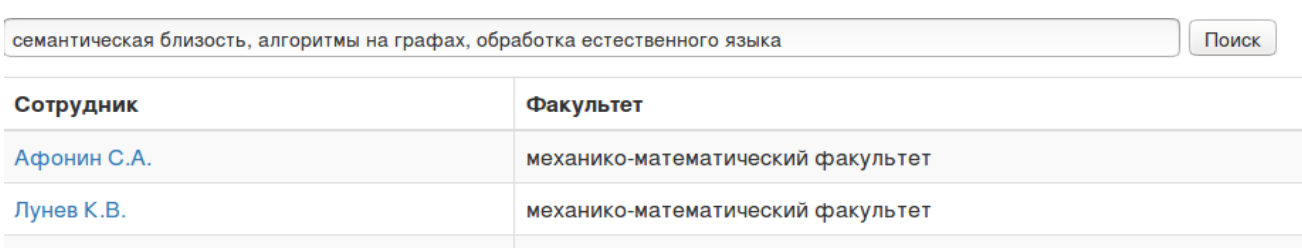
\includegraphics[width=0.95\linewidth]{Dissertation/pics/search}
    \caption{Интерфейс модуля поиска по ключевым словам}
  \end{minipage}
  \label{img:search}
\end{figure}

Помимо этого реализовано ядро подсистемы обработки ключевых слов, которое проводит основной анализ, определение семантической близости пары слов, подготовку тезауруса ключевых слов. Методы определения сематнической близости пары ключевых слов описаны в главе \ref{chapt1}, а описание алгоритма построения тезауруса дано в разделе \ref{thes}. Код ядра представляет собой модули, процедуры и скрипты на языке Python с использованием открытых математических пакетов (Numpy, Pandas, Scipy), а также пакетов для анализа данных и машинного обучения (Scikit-learn, XGBoost). Данный модуль может использоваться отдельно от основного кода системы.

\begin{figure}[ht]
  \begin{minipage}[ht]{1.0\linewidth}\centering
    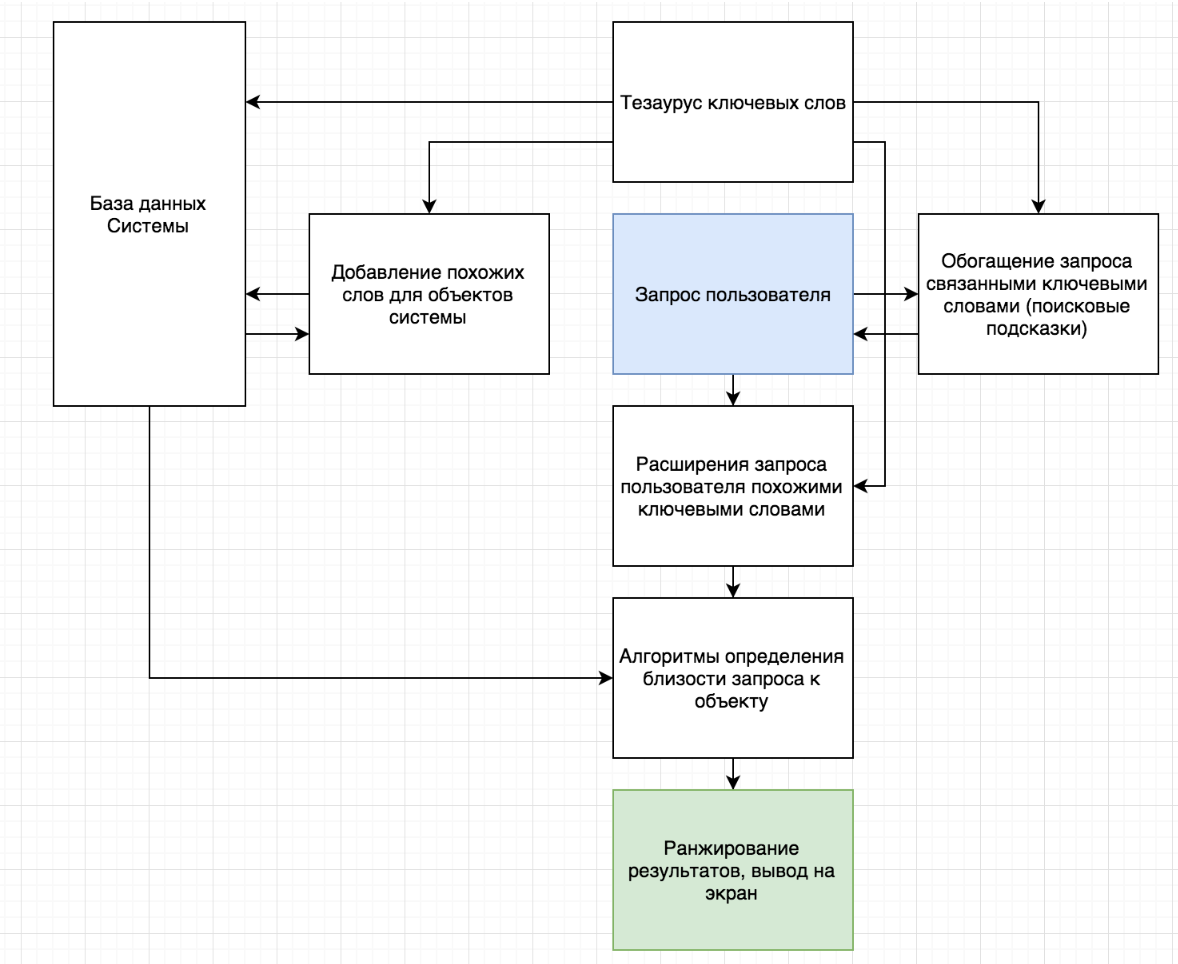
\includegraphics[width=0.95\linewidth]{Dissertation/pics/search_2}
    \caption{Схема обработки запроса на поиск по ключевым словам}
  \end{minipage}
  \label{img:search_2}
\end{figure}

На рис.\ref{img:search_2} представлена схема выполнения и обработки запроса. Основной процесс работы с ключевыми словами состоит из трех шагов. На первом из них в ядре модели рассчитывается тезаурус ключевых слов. В этом тезаурусе для каждого ключевого слова хранятся ключевые слова, близкие по смыслу к данному, с указанием значения меры близости. Далее полученный словарь загружаются в базу данных системы, после чего появляется возможность по введенному пользователем слову быстро восстанавливать множество ключевых слов, похожих на заданное. Данный этап сбора словаря стоит обособленно от процесса поиска и может быть перезапущен в любой момент времени. 

Второй шаг - обогащение объектов системы ключевыми словами из собранного на прошлом шаге тезауруса. Если для объекта указан набор ключевых слов, то для к каждому из этих ключевых слов добавляется информация о близких словах из тезауруса. Данный этап также является шагом предобработки данных. 

Последний этап - непосредственно поиск по ключевым словам. Введенный пользователем запрос расширяется словами тезауруса, далее происходит поиск сущностей по расширенным наборам ключевых слов (как в запросе, так и в описании объекта). Для найденных объектов вычисляется релевантность (функция, возвращающая действительное число по паре запрос-объект, большие значения которой соответствуют более релевантным объектам), результаты сортируются по убыванию релевантности и выводятся на экран пользователя. Использование поискового запроса пользователя как набора ключевых слов, позволяет применять упомянутые выше алгоритмы для разработки поисковых подсказок. Такие подсказки предлагают пользователю дополнить свой запрос ключевыми словами, связанными по смыслу с теми, которые он уже ввел.

Трудностью в решении задачи реализации поиска по ключевым словам является тот факт, что для значительной части слов в системе нет достаточной статистики их использования. Как следствие, возникает ситуация, когда про слово, добавленное к описанию объекта или про слово, заданное пользователем в поисковую строку, нет достаточной информации, что не позволяет получить релевантную запросу поисковую выдачу. Для преодоления этой трудности в системе реализованы интеллектуальные алгоритмы анализа ключевых слов, а также используются внешние корпусы данных на естественном языке, описанные в разделе \ref{ml_sim}. Основными направлениями работы по использованию ключевых слов для выполнения поисковых запросов являются следующие:

\begin{itemize}
    \item определение семантической близости между парой ключевых слов с помощью алгоритмов машинного обучения и внешних наборов данных;
    \item определение семантической между парами наборов ключевых слов;
    \item использование связей между объектами системы (например, списки публикаций одного автора, таблицы соавторства, списки участников конференции, работников лаборатории и др.)
\end{itemize}

Таким образом, поиск по ключевым словам осуществляет не только определение точного вхождения слов запроса в слова объектов, по которым ведется поиск, но также происходит расширение как запроса, так и подлежащих анализу документов семантически близкими словами. В дополнении к этому, наборы ключевых слов, ассоциированные с объектами системы, обогащаются словами, от связанных с ними объектов. Все это позволяет увеличить описание к имеющимся данным и, следовательно, улучшить возможности поиска. 


\subsection{Поисковые подсказки для ключевых слов}
Поисковые подсказки позволяют облегчить пользователю формулировку запроса к системе на естественном языке. Стандартные алгоритмы построения поисковых подсказок позволяют выбрать необходимое слово по его введенному префиксу. Но во многих ситуациях является важным подсказать пользователю слово, близкое по значению к вводимому. Такое слово пользователь, возможно, не вспомнил во время ввода запроса. Алгоритм полезен также и в тех случаях, когда пользователь планировал ввести предлагаемое слово, поскольку это экономит время ввода: нет необходимости полностью вводить слово, его можно просто выбрать из списка предложенных слов.

Поэтому была реализована система поисковых подсказок, описание которой приведено далее:
\begin{itemize}
    \item известные системе ключевые слова кладутся в префиксное дерево;
    \item в листья префиксного дерева кладутся ссылки на ключевые слова, близкие к слову, построенному от вершины дерева до этого листа;
    \item при вводе пользователем слова, в интерфейсе появляется список возможных завершений данного слова, построенный обходом от текущей вершины в префиксном дереве;
    \item при достижении листовой вершины (путем полного ввода слова или выбора подсказки) в интерфейсе показывается список слов, близких по смыслу к только что введенному. Слова этого списка отсортированы по уменьшению значения функции семантической близости;
    \item при выборе одного из слов из списка семантически близких к введенному, это слово добавляется в запрос. Пользователю предлагается выбрать близкие слова к только что добавленному или начать вводить следующее слово самостоятельно.
    \item при нажатии на кнопку <<Поиск>> начинается процесс построения поисковой выдачи по введенному запросу.
\end{itemize}
        
\section{Выводы}
%\
